\documentclass{sig-alternate}

\usepackage[utf8]{inputenc}
\usepackage{xspace}
\usepackage[ampersand]{easylist}
\usepackage{qtree}
\usepackage{color}


\newtheorem{definition}{Definition}
\newtheorem{proposition}{Proposition}



\newenvironment{lizt}
{\begin{easylist}[itemize]}
{\end{easylist}}

\newcommand{\superscript}[1]{\ensuremath{^{\textrm{#1}}}}
\def\sharedaffiliation{\end{tabular}\newline\begin{tabular}{c}}

\def\wu{\superscript{*}}
\def\wg{\superscript{\dag}}

\newcommand{\Lets}{Let us\xspace}
\newcommand{\lets}{let us\xspace}
\newcommand{\lterm}{$\lambda$-term\xspace}
\newcommand{\lterms}{$\lambda$-terms\xspace}
\newcommand{\lhead}{$\lambda$-head\xspace}
\newcommand{\lheads}{$\lambda$-heads\xspace}
\newcommand{\la}{\leftarrow\xspace}
\newcommand{\Lp}  {\Lambda^{\prime}\xspace}
\newcommand{\tur}[3]{#1\vdash{}#2 \colon #3}
\newcommand{\turst}[3]{$#1\vdash{}#2:#3$\xspace}
\newcommand{\GMS}{\turst{\Gamma}{M}{\sigma}}
\newcommand{\atTree}{@-tree\xspace}
\newcommand{\setDots}[2]{ \lbrace #1 , \dots , #2 \rbrace}
\newcommand{\lh}[1]{\lambda #1}
\newcommand{\sexprTree}{sexpr-tree\xspace}
\newcommand{\SexprTree}{Sexpr-tree\xspace}
\newcommand{\then}{\Rightarrow\xspace}
\newcommand{\lamb}[2]{( \lambda \, #1 \, . \, #2 )}
\newcommand{\lam}[2]{\lambda \, #1 \, . \, #2}
\newcommand{\ST}{\mathop{\mathrm{ST}}}
\newcommand{\FV}{\mathop{\mathrm{FV}}}
\newcommand{\Scomb }{\mathbf{S}}
\newcommand{\Kcomb }{\mathbf{K}}
\newcommand{\Icomb }{\mathbf{I}}
\newcommand{\bbarr}{\twoheadrightarrow_\beta}
\newcommand{\barr}{\rightarrow_\beta}
\newcommand{\beq}{=_\beta}
\newcommand{\eearr}{\twoheadrightarrow_\eta}
\newcommand{\earr}{\rightarrow_\eta}
\newcommand{\eeq}{=_\eta}
\newcommand{\bearr}{\rightarrow_{\beta\eta}}
\newcommand{\bbeearr}{\twoheadrightarrow_{\beta\eta}}
\newcommand{\beeq}{=_{\beta\eta}}
\newcommand{\etar}{\twoheadrightarrow_\eta}
\newcommand{\ered}{$\eta$-reduction\xspace}
\newcommand{\bnf}{$\beta$-\textit{nf}\xspace}
\newcommand{\enf}{$\eta$-\textit{nf}\xspace}
\newcommand{\eenf}{$\eta^{-1}$-\textit{nf}\xspace}
\newcommand{\beenf}{$\beta\eta^{-1}$-\textit{nf}\xspace}
\newcommand{\benf}{$\beta\eta$-\textit{nf}\xspace}
\newcommand{\bredex}{$\beta$-redex\xspace} 
\newcommand{\lnf}{\textit{lnf}\xspace}
\newcommand{\Ae}{\mathop{\mathrm{\AE}}}
\newcommand{\Bcomb }{\mathbf{B}}   
\newcommand{\BBcomb }{\mathbf{B*}}
\newcommand{\Ccomb }{\mathbf{C}}   
\newcommand{\CCcomb }{\mathbf{C'}}
\newcommand{\SScomb }{\mathbf{S'}}
\newcommand{\ar}{\rightarrow\xspace}
\newcommand{\T}{\mathbb{T}\xspace}
\newcommand{\C}{\mathbb{C}\xspace}
\newcommand{\Real}{\mathbb{R}}
\newcommand{\gar}{\longmapsto}
\newcommand{\bRedex}{$\beta$-redex\xspace}
\newcommand{\bRedexes}{$\beta$-redexes\xspace}
\newcommand{\bArrow}{\rightarrow_\beta\xspace}
\newcommand{\eArrow}{\rightarrow_\eta\xspace}
\newcommand{\eeArrow}{\rightarrow_{\eta^{-1}}\xspace}


\newenvironment{todo}
{~\\ {\color{red}\textbf{TODO}}
  \begin{easylist}[itemize]}
{ \end{easylist}}

\newcommand{\Lpr}{\Lambda^\prime}
\newcommand{\ul}[2]{\langle #1 ; #2 \rangle}
\newcommand{\ro}[1]{{\color{blue} #1}}
\newcommand{\tom}[1]{{\color{ForestGreen} #1}}
\newcommand{\red}[1]{{\color{red} #1}}
\newcommand{\nehodi}[1]{{\color{yellow} #1}}



\begin{document}

\conferenceinfo{GECCO'14,} {July 12-16, 2014, Vancouver, BC, Canada.}
\CopyrightYear{2014}
\crdata{TBA}
\clubpenalty=10000
\widowpenalty = 10000

\title{Utilization of Reductions and Abstraction Elimination in Typed Genetic Programming}


% \numberofauthors{2} 
%
%  \author{
%  % 1st. author
%  \alignauthor
%  Tom\'{a}\v{s} K\v{r}en\\
%    \affaddr{Faculty of Mathematics and Physics}\\
%    \affaddr{Charles University in Prague}\\
%    \affaddr{Malostransk\'e n\'am\v{e}st\'\i~25, 11000,}\\
%    \affaddr{Prague, Czech Republic}\\
%    \email{tomkren@gmail.com}
%  % 2nd. author
%  \alignauthor
%  Roman Neruda\\
%    \affaddr{Institute of Computer Science}\\
%    \affaddr{Academy of Sciences of the Czech Republic}\\
%    \affaddr{Pod Vod\'arenskou v\v{e}\v{z}\'\i~2, 18207,}\\
%    \affaddr{Prague, Czech Republic}\\
%    \email{roman@cs.cas.cz}
%  }

\numberofauthors{2}
\author{
  \alignauthor \ Tom\'{a}\v{s} K\v{r}en\wu\wg\\
  \email{tomkren@gmail.com}
  %
  \alignauthor \ Roman Neruda\wu\\
  \email{roman@cs.cas.cz}
  %
  \sharedaffiliation
  \begin{tabular}{ccc}
    \affaddr{{\wu}Institute of Computer Science{\ }}      & & \affaddr{{\wg}Faculty of Mathematics and Physics{\ }} \\
    \affaddr{Academy of Sciences of the Czech Republic}   & & \affaddr{Charles University in Prague} \\
    \affaddr{Pod Vod\'arenskou v\v{e}\v{z}\'\i~2, 18207,} & & \affaddr{Malostransk\'e n\'am\v{e}st\'\i~25, 11000,} \\
    \affaddr{Prague, Czech Republic}                      & & \affaddr{Prague, Czech Republic} \\
  \end{tabular}
}



%\date{24 January 2014}

\maketitle
\begin{abstract}
Lambda calculus representation of programs offers a more expressive alternative to traditional S-expressions. In this paper we discuss advantages of this representation coming from the use of reductions (beta and eta) and a way to overcome disadvantages caused by variables occurring in the programs by use of the abstraction elimination algorithm. We discuss the role of those reductions in the process of generating initial population and propose several crossover approaches, two of which are based on abstraction elimination and compared using the even parity benchmark problem.
\red{Přidat víc o kříženích tak aby davál insight to the project.}
%including novel approach to crossover operator based both on reductions and abstraction elimination. 
%The design goal of this operator is to turn the disadvantage of abstraction elimination  - possibly quadratic increase of program size - into a virtue; our approach leads to more crossover points. At the same time, utilization of reductions provides offspring of small sizes.
\end{abstract}

%Starej abstrakt než se zjistilo že unpacking neni tak super:
%Lambda calculus representation of programs offers a more expressive alternative to traditional S-expressions. In this paper we discuss advantages of this representation coming from use of reductions (beta and eta) and how to overcome disadvantages caused by variables occurring in the programs by use of the abstraction elimination algorithm. We discuss the role of those reductions in the process of generating initial population and compare several crossover approaches including novel approach to crossover operator based both on reductions and abstraction elimination. The design goal of this operator is to turn the disadvantage of abstraction elimination  - possibly quadratic increase of program size - into a virtue; our approach leads to more crossover points. At the same time, utilization of reductions provides offspring of small sizes.


% A category with the (minimum) three required fields
\category{I.2.2}{Artificial Intelligence}{Automatic Programming}[Program synthesis]
%A category including the fourth, optional field follows...
\category{F.4.1}{Mathematical Logic and Formal Languages}{Mathematical Logic}[Lambda calculus and related systems]

\terms{Experimentation, Languages, Theory}

\keywords{genetic programming, lambda calculus}

\section{Introduction}


Genetic programming (GP) represents an efficient method for automatic generating of programs by means of evolutionary techniques~\cite{koza92,koza03}. Early attempts to enhance the GP approach with the concept of types include the seminal work~\cite{montana95} where the ideas from Ada programming language were used to define a so-called strongly typed GP.   
Usage of types naturally opens door to enriching S-expressions,
the traditional GP representation of individuals, with concepts from
lambda calculus, which is a simple yet powerful functional, mathematical and programming language extensively used in type theory. Such attempts have shown to be successful \cite{yu01}. 

One of the motivations for using lambda calculus is that it is backed by a considerable theoretical background. From this background we can utilize several useful concepts such as reductions, normalization or abstraction elimination, and use them to enhance the standard GP algorithm. We use normalization to reduce the size of the search space of program trees and the abstraction elimination to prevent
the difficulties caused by the presence of variables in program trees.

In our system we use simply typed lambda calculus. Since abstraction elimination and reductions do not involve many type related issues it seems to us as a sufficient choice of type system. Techniques described here would be analogous for a more sophisticated type system and can be directly applied to such systems as the Hindley–Milner type system.


\red{Zdůraznit že main contribution of this paper je popis crossover operations který [rekapitulovat dobrý vlastnosti našeho křížení z 2ky (a dalších sekcí), tj že to nezjednodušuje na méně obecnou notaci a přesto to zůstává efektivní i v problémech kde to zjednodušení hraje do karet tý metodě.]}

%\red{Možná někam poznamenat že přínos toho článku je taky v tom že zpřístupňuje pojmy z teorie typovaného lc komunitě typovaného GP esli to neni blbý..}

%Pro inspiraci :
%\nehodi{The key issue in the lambda calculus approach to enrich GP with types is the method of individual generation. During the expansion phase the set of unfinished terms can be browsed with respect to various search strategies. Our approach to this problem aims to utilize the full arsenal given by the simply typed lambda calculus. Thus, the natural idea is to employ an exhaustive systematic search. On the other hand, if we were to mimic the standard GP approach, a quite arbitrary yet common and successful ramped half-and-half generating heuristic~\cite{fg} should probably be used. These two search methods in fact represent boundaries between which we will try to position our parameterized solution that allows us to take advantage of both strategies. This design goal also differentiate our approach from the three state of the art proposals for typed GP known to us that are discussed in the following section. Our proposed \emph{geometrical search strategy} described in this paper is such a successful hybrid mixture of random and systematic exhaustive search. Experiments show that it is also very efficient dealing with one of the traditional GP scarecrows - the bloat problem.}

The rest of the paper is organized as follows: The next section briefly discusses related work in the field of typed GP, while section~\ref{preliminaries} introduces necessary notions.
The body of the paper is presented in sections \ref{generating} and \ref{crossover}; the first discusses the term generating 
procedure and its relations
with reductions, the second describes several approaches to lambda term
crossover and how they solve the variable problem. Section~\ref{experiments} examines those ideas on the even parity benchmark problem, while the paper is concluded by section~\ref{conclusions}.

\section{Related work}
\label{related}

Yu presents a GP system utilizing
polymorphic higher-order functions\footnote{Higher-order 
function is a function taking another function as 
input parameter.} and lambda abstractions  \cite{yu01}.
An important point of interest in the work is use of
\texttt{foldr} function as a tool for \textit{implicit recursion}, i.e. recursion without explicit recursive calls. The terminal set for constructing lambda abstraction subtrees  is limited to use only constants and variables of that particular lambda abstraction, i.e., outer variables are not allowed to be used as terminals in this work. This is a significant difference from our approach since we permit all well-typed normalized \lterms. This difference also causes the need for different crossover operators.  

Briggs and O’Neill present a technique 
utilizing typed GP with combinators \cite{kes}.
The difference between approach presented in their work
and our approach is that they generate terms in a straightforward way directly from the library of combinators, without any use of lambda abstractions. They use the Hindley–Milner type system. They also present interesting concept of \textit{Generalized genetic operator} based on term generation. The combinator based genetic algorithm has the advantage of
avoiding the need of dealing with variables.

Binard and Felty use even stronger type system (\textit{System F}) \cite{binard2008genetic}. But with the increasing power of the type system also comes an increasing difficulty of term generation. For this reason, the evolution in this work takes interesting and nonstandard shape (fitness is associated with \textit{genes} which are evolved together with \textit{species} which together participate in creation of individuals). This differs from our approach, which tries to be a generalization of the standard GP\cite{koza92}.

In contrast with the above mentioned works, our approach uses very simple type system (simply typed lambda calculus) and concentrates on process of generation  
able to generate all possible well-typed normalized lambda terms. In order to do so we use technique based on \textit{inhabitation machines} described by Barendregt \cite{barendregt10}.    

\section{Preliminaries}
\label{preliminaries}

\red{Buď přidat neformální komentář a/nebo odebrat nadbytečný věci.}

In this section, several notions necessary to build a typed GP based on lambda calculus are introduced. 
First, \lets describe a programming language, 
in which the GP algorithm generates individual programs --- the so called \lterms.

\begin{definition}
Let $V$ be infinite countable set of {\it 
variable names}. Let $C$ be set of {\it constant names}, 
$V \cap C = \emptyset$.	 	
Then $\Lambda$ is set of {\it \lterms} defined inductively as follows.	
\begin{align*}
x   \in V \cup C  &\then x     \in \Lambda \\
M,N \in \Lambda   &\then (M~N) \in \Lambda 
\textit{~~~~~~(Function application)} \\
x   \in V , M \in \Lambda &\then \lamb{x}{M} \in \Lambda
\textit{~~~~($\lambda$-abstraction)} 
\end{align*}
\end{definition}


\textit{Function application} and 
\textit{$\lambda$-abstraction} are concepts
well known from common programming languages. 
For example, in JavaScript, 
$(M~N)$ translates to expression \texttt{$M$($N$)} and
$\lamb{x}{M}$ translates to expression \texttt{function($x$)\{return $M$;\}}.
In other words, the function application 
corresponds to the act of supplying a function 
with an argument, and
the $\lambda$-abstraction is equivalent to 
\textit{anonymous function}\footnote{Apart from JavaScript, anonymous functions are common e.g. in Python and Ruby, 
they were recently introduced to C++, and they are expected to be supported in Java 8.}.

For better readability, 
$M_1~M_2~M_3~\dots~M_n$ will be an abbreviation for
$(\dots((M_1~M_2)~M_3)~\dots~M_n)$,
and $\lam{x_1 x_2 \dots x_n }{M}$ will be an abbreviation for 
$\lamb{x_1}{\lamb{x_2}{\dots\lamb{x_n}{M}\dots}}$.


\subsection{Reductions}

In order to perform computation, there must be some
mechanism for term evaluation. In $\lambda$-calculus there
is a \mbox{$\beta$-reduction} procedure for this reason.\\

A term of a form $\lamb{x}{M}N$ is called \textit{\bRedex}.
A \bRedex can be $\beta$-reduced to term $M[x:=N]$. 
This fact is written as \textit{relation} $\bArrow$ 
of those two terms:
\begin{equation} \label{eq:bRed}
\lamb{x}{M}N \bArrow M[x:=N]
\end{equation}
It is also possible to reduce \textit{subterm \bRedexes} 
which can be formally stated as:
\begin{align*}
P \bArrow Q &\then (R~P)      \bArrow (R~Q) \\
P \bArrow Q &\then (P~R)      \bArrow (Q~R) \\
P \bArrow Q &\then \lam{x}{P} \bArrow \lam{x}{Q}  
\end{align*}

In other words, $\beta$-reduction is the process 
of insertion of arguments supplied to a function into 
its body. \\

Another useful relations are $\bbarr$ and $\beq$ defined as follows. 

\begin{enumerate}
 \item \begin{enumerate}
 	\item $M \bbarr M$
 	\item $M \barr N \then M \bbarr N$
 	\item $M \bbarr N , N \bbarr L \then M \bbarr L$ 	
 \end{enumerate}
 \item \begin{enumerate}
 	\item $M \bbarr N \then M \beq N$
 	\item $M \beq N \then N \beq M$
 	\item $M \beq N , N \beq L \then M \beq L$
 \end{enumerate}

\end{enumerate}

We read those relations as follows.
\begin{enumerate}
 	\item $M \bbarr N$ --- "$M$ $\beta$-reduces to $N$."  
 	\item $M \barr N$  --- "$M$ $\beta$-reduces to $N$
 	      in one step."
 	\item $M \beq N$ --- "$M$ is $\beta$-convertible to $N$."	
 \end{enumerate}


Similarly as for $\beta$-reduction we can define $\eta$-reduction except that now it is defined as follows.  
$$\lamb{x}{(M~x)} \eArrow M \textbf{ ~~~~if } x \not\in FV(M) $$

Analogically, a term of a form $\lamb{x}{(M~x)}$ is called 
\textit{$\eta$-redex}.

Relation $\bearr\;=\;\barr \cup \earr$. 
(Relation $R = \{\;(a,b)\;|\;a\;R\;b\;\}$.)
Similarly as for $\bbarr$ and $\beq$ we can define relations 
$\eearr$, $\eeq$,$\bbeearr$ and $\beeq$.\\

$\eta^{-1}$-reduction (also called $\eta$-expansion) is 
the reduction converse to $\eta$-reduction.
It is defined as follows.  
$$M \eeArrow \lamb{x}{(M~x)} \textbf{ ~~~~if } x \not\in FV(M) $$


\subsection{Normal forms}
\begin{definition}~

\begin{easylist}[enumerate]
& A \lterm is a \textit{$\beta$-normal form} (\bnf) 
if it does not have a $\beta$-redex as subterm.
& A \lterm M \textit{has} a \bnf if $M \beq N$
and $N$ is a \bnf.\\
\end{easylist}
\end{definition}
A normal form may be thought of as a result of a term evaluation. 
Normalization of the term $M$ is the process of finding normal form of $M$. 

Similarly we can define \enf and \benf.

\subsection{Types}

A \lterm as described above
corresponds to a program expression with no type information
included. Now we will describe \textit{types} (or \textit{type terms}).

\begin{definition}
Let $A$ be set of {\it atomic type names}. 
Then $\mathbb{T}$ is set of {\it types} inductively defined as follows.
\begin{align*}
\alpha      \in A  &\then   \alpha \in \T \\
\sigma,\tau \in \T &\then ( \sigma \ar  \tau ) \in \T 
\end{align*}
\end{definition}


Type $\sigma \ar \tau$ is type for functions taking as input
something of a type $\sigma$ and returning 
as output something of a type $\tau$. 
$\tau_1 \ar \tau_2 \ar \dots \ar \tau_n$ is an abbreviation for 
$\tau_1 \ar (\tau_2 \ar (\dots \ar (\tau_{n-1} \ar \tau_n)\dots))$.
The system called \textit{simply typed $\lambda$-calculus} is now easily obtained by
combining the previously defined \textit{\lterms} and \textit{types} together.

\begin{definition}~

\begin{enumerate}
 \item 	Let $\Lambda$ be set of {\it \lterms}. 
	Let $\mathbb{T}$ be set of {\it types}.       
	A {\it statement} $M : \sigma$ is a pair 
	$(M,\sigma) \in \Lambda \times \mathbb{T}$.
	Statement $M : \sigma$ is vocalized as 
	{\it "$M$ has type $\sigma$"}.
	The term $M$ is called the {\it subject} of the 
	statement $M : \sigma$.
 \item A \textit{declaration} is a statement 
 $x : \sigma$ where $x \in V \cup C$.
  
 \item A \textit{context} 
 is set of declarations with distinct variables as subjects.
\end{enumerate}
\end{definition}
%~\\

Context is a basic type theoretic concept suitable as a typed alternative
for terminal, and function set in standard GP. 
Notation $\Gamma,x:\sigma $ denotes $ \Gamma\cup\{(x:\sigma)\}$ 
such that $\Gamma$ does not contain any declaration with $x$ as subject.
We also write $x:\sigma \in \Gamma$ instead of $(x,\sigma) \in \Gamma$.

\begin{definition}
A statement $M\colon\sigma$ is \textit{derivable from}
a context $\Gamma$ (notation 
\mbox{$\Gamma\vdash{}M\colon\sigma$}) 
if it can be produced by the following rules.
\begin{align*}
x : \sigma \in \Gamma &~\then~ \tur{\Gamma}{x}{\sigma}\\
\tur{\Gamma}{M}{\sigma \ar \tau}~,~\tur{\Gamma}{N}{\sigma} 
&~\then~ \tur{\Gamma}{(M~N)}{\tau}\\  
\tur{\Gamma,x:\sigma}{M}{\tau}
&~\then~ \tur{\Gamma}{\lamb{x}{M}}{\sigma \ar \tau} 
\end{align*}
\end{definition}

Our goal in term generation is to produce terms $M$
for a given pair $\ul{\tau}{\Gamma}$
such that for each $M$ is $\tur{\Gamma}{M}{\tau}$.

\subsection{Long normal form}
\label{lnf}

%v barendrechtovi je to v definici lnf
%$\lam{x_1 \dots x_n}{f~M_1~\dots~M_n}$ místo $M_m$ 
%ale to musí bejt určitě překlep...

\begin{definition}
Let \GMS where 
$\sigma = \tau_1 \ar \dots \ar \tau_n \ar \alpha, n \geq 0$.
	\begin{enumerate}
	  \item	
		Then $M$ is in \textit{long normal form} (\lnf) if following 
		conditions are satisfied.
		\begin{enumerate}
		 \item $M$ is term of the form $\lam{x_1 \dots x_n}{f~M_1~\dots~M_m}$\\
		  (specially for $n = 0$, $M$ is term of the form $f$).
		 \item Each $M_i$ is in \lnf.
		\end{enumerate}	
	  \item 
	    $M$ has a \lnf if $M =_{\beta\eta} N$ and $N$ is in \lnf.
	\end{enumerate}
\end{definition}~

As is shown in \cite{barendregt10}, \lnf has following nice properties.

\begin{proposition}
If $M$ has a \bnf, 
%which according to Theorem 2B.4 is always the case, 
then it also has a unique \lnf, 
which is also its unique \beenf.
\end{proposition}

\begin{proposition}
Every $B$ in \bnf has a \lnf 
$L$ such that $L \twoheadrightarrow_{\eta} B$.
\end{proposition}

\subsection{Abstraction elimination}

\textit{Abstraction elimination} is a process of transforming 
an arbitrary \lterm into \lterm that contains no lambda abstractions
and no bound variables.
The newly produced \lterm may contain function applications, 
free symbols from former \lterm and some new symbols standing for 
combinators $\Scomb$, $\Kcomb$ and $\Icomb$. \\

Those combinators are defined as:
\begin{align*}
\Scomb &= \lam{f\,g\,x}{f\,x\,(g\,x)} \\
\Kcomb &= \lam{x\,y}{x} \\
\Icomb &= \lam{x}{x} 
\end{align*}


\Lets describe transformation $\Ae$ performing this 
process.
%\footnote{In our implementation we must also deal with types, because our individuals are annotated with types. But since this process is fairly straightforward but cumbersome to describe, we will skip explaining it here. Reader interested in seeing it can see the source code of our implementation. }
\begin{align*}
\Ae[x]           &= x &\\[0.4em]
\Ae[\,(M\,N)\,]  &= (\Ae[M]\;\;\Ae[N]) &\\[0.4em]
\Ae[\lam{x}{x}]  &= \Icomb &\\
\Ae[\lam{x}{M}]  &= (\Kcomb~\Ae[M]) &\textbf{if } x \not\in \FV(M)\\
\Ae[\lam{x}{\lamb{y}{M}}] &= \Ae[\lam{x}{\Ae[\lam{y}{M}]}]  
&\textbf{if } x \in \FV(M)\\
\Ae[\lam{x}{(M\,N)}] &= (\Scomb~\Ae[\lam{x}{M}]~\Ae[\lam{x}{N}])  
&\textbf{if } x \in \FV(M)\\
&&\vee~ x \in \FV(N)\\
\end{align*}

As is stated in \cite{jones87},
the biggest disadvantage of this technique is that the translated
term is often much larger than in its lambda form --- the size of
the translated term can be proportional to the square of the size 
of the original term. But the advantage is also tempting --- no need to deal with variables and lambda abstractions.

The algorithm presented here is a simple version of this process. 
More optimized version (used in our \textit{hybrid} crossover described below), by means of the size of resulting term and its time performance is presented in \cite{jones87}. 

\section{Term generating and reductions}
\label{generating}

This section is focused on the individual generating method producing
terms in their long normal form, which can be understood as a straight 
generalization of S-expressions into lambda calculus. 
We discuss the relation between terms in \lnf with beta and eta reductions,
the advantages of such representation and we also show how to easily 
transform such terms into short \benf.
   
\subsection{Grammar producing \lterms in \lnf}

In \cite{barendregt10}, the following term generating 2-level grammar\footnote{2-level grammar (unlike a standard grammar) can have infinitely many non-terminals and its rule is better described as \textit{rule schema}. The original grammar described in \cite{barendregt10} has $( \sigma \rightarrow \tau , \Gamma ) \gar (~\lambda~x~.~( \tau ; \Gamma,x:\sigma )~)$ as second rule, but our grammar is equivalent -- it packs consecutive uses of this rule into our rule.} for generating all possible
terms in their \textit{long normal form} is described.

If we want to generate a term $M$ satisfying $\tur{\Gamma}{M}{\tau}$,
then the initial non-terminal is $(\tau, \Gamma)$.

For every $\alpha \in A$ and context $\Gamma$ and $f$ such that \\
$(f :$ $\rho_1 \ar \dots \ar \rho_m \ar \alpha$ $) \in \Gamma$ 
we have a rule of the first form:
$$
( \alpha , \Gamma ) \gar 
(~f~( \rho_1 , \Gamma )~\dots~( \rho_m , \Gamma )~)
$$

In other words, one possible way to construct a term of 
the atomic type $\alpha$ from the building symbols $\Gamma$
is to take a function symbol $f$ from $\Gamma$ with 
the return type $\alpha$ (or if $m=0$ a constant of the type $\alpha$),
put it into the root of the term and to generate 
a subtrees of appropriate types for each of $f$'s arguments
from the building symbols $\Gamma$.  

For every atomic type $\alpha$, context $\Gamma$ and types
$\tau_1 , \dots , \tau_n$ (where $n > 0$) 
we have a rule of the second form:\\

$
( \tau_1 \ar \dots \ar \tau_n \ar \alpha , \Gamma )  
 \\ ~~~~~~~~\gar
(~\lambda~x_1~\dots~x_n~.~
( \alpha ; \Gamma , x_1:\tau_1 , \dots , x_n:\tau_n  )~)
$~\\

In other words, the way to construct a term of 
the function type $\tau_1 \ar \dots \ar \tau_n \ar \alpha$ 
from the building symbols $\Gamma$
is to create an anonymous function
with fresh variables $x_1, \dots , x_n$ in its head 
whose body is constructed as a term that has type $\alpha$
and is constructed using symbols from $\Gamma$ 
enriched with those new variables $x_1, \dots , x_n$,
which are associated with appropriate types.
  

% TODO dyštak zmínit že sme druhý pravidlo nahradili fikanou zkratkou
%The second rule can be replaced by more effective one.
%This rule packs consecutive uses of the second rule into one use. This is valid since the use of the second rule is deterministic; it is used if and only if the non-terminal's type is not atomic.

Long normal form is a generalization of S-expressions into lambda calculus:
Let $\Gamma$ be a context satisfying the closure requirement, then only
the first rule will be applicable. 
$(\alpha, \Gamma)$ rewrites to $(~f~( \alpha, \Gamma )~\dots~( \alpha, \Gamma )~)$.
One can see that $f$ stands for 
the root node and that each $( \alpha , \Gamma )$ will produce a direct subtree. 

For a context containing at least one higher order function 
(or if the desired type of generated terms is a function type) we get special kind of root node containing lambda head with one direct subtree standing for body of the lambda function. Local variables defined in the lambda head may also appear in this body. 


Discussion of what is the best strategy for browsing the search space given by above described grammar in order to generate \lnf terms is beyond the scope of this paper. Standard \textit{ramped half-and-half} strategy can be used for this purpose, or some other, 
which we discuss in \cite{nasecec}. In our experiments we use the \textit{geometric} strategy proposed in 
\cite{nasecec}.


\subsection{Benefits of generating \lterms in \lnf}
\label{benefits}

By generating \lterms in \textit{lnf} we avoid generating 
\lterms $M$,$N$ such that $M \not= N$, but $M =_{\beta\eta} N$.
In other words, we avoid generating two programs with different 
source codes, but performing the same computation.
\red{Zde potřeba doplnit vysvětlení, že to řeší jen čast tohoto
fenomenu}


Every \lterm $M$ such that \GMS has its unique \lnf $L$, 
for which $L =_{\beta\eta} M$.
Therefore, the computation performed by \lterm $M$ 
is not omitted, because it is the same computation
as the computation performed by \lterm $L$. \\

Generating \lterms in \lnf is even better than generating 
\lterms in \bnf. Since \lnf is the same thing as \beenf,
every \lterm in \lnf is also in \bnf. 

This comes straight from the definition of \beenf, 
but one can also see it by observing the method for generating
terms in \bnf. As shown in \cite{barendregt10}, 
this method is obtained by the following 2-level grammar.
\begin{align*}
( \pi , \Gamma )  
&\gar
(~f~( \rho_1 , \Gamma )~\dots~( \rho_m , \Gamma )~)
\\ 
( \sigma \rightarrow \tau , \Gamma )  
&\gar
(~\lambda~x~.~( \tau ; \Gamma,x:\sigma )~)
&   
\\& \textit{where~~~} (f : \rho_1 \ar \dots \ar \rho_m \ar \pi) \in \Gamma
\end{align*}

This grammar differs from the grammar for \lnf only in the first rule\footnote{We use a different second rule for \lnf grammar, but as is mentioned in footnote above, it also works with this second rule.}. Specifically, it differs in that $f$'s type is no longer needed to be fully expanded ($\pi \in \T$ instead of $\alpha \in A$). This makes the grammar less deterministic,
resulting in a bigger search space. The new rule is generalization of the old one,
thus all terms in \lnf will be generated, along with many new terms in \bnf that 
are not in \lnf. 
    
By generating \lterms in \lnf we avoid generating 
\lterms $M$,$N$ such that $M \not= N$ and $M =_{\eta} N$; 
but generating in \bnf does not have such a property..\\


The disadvantage of the \lnf, as the name suggests, is that it is long.
Terms in \lnf are said to be \textit{fully $\eta$-expanded} \cite{barendregt10}. 
A relevant property of $\eta$-reduction is that it always shortens the term
that is being reduced by it. And conversely, $\eta$-expansion prolongs.
$$\lamb{x}{(M~x)} \eArrow M \textbf{ ~~~~if } x \not\in FV(M) $$

Now we show that for every \lterm $M$, 
every sequence of $\eta$-reductions is finite and
it leads to a unique \enf $N$.

\begin{enumerate}
 \item Every application of \ered shortens the term.
       Since every term has finite size, this process must 
       end at some point. Thus every \lterm has \enf.
 \item Since \ered is \textit{Church–Rosser}, \enf is unique (see~\cite{barendregt84}). 
\end{enumerate}

So we can take every generated \lterm $M$ in 
\lnf and transform it to shorter term in \enf. 
The question is whether it remains in \bnf, thus being in \benf.
The answer is yes; it can be proven by showing that no 
new \bredex is created by \ered.  

\begin{proposition}
Let $P$ be in \bnf and $P \eArrow Q$. Then $Q$ is in \bnf.    
\end{proposition}
\begin{proof}

For better clarity \lets show the \ered and \bredex using \atTree{}s 
(a \lterm representation derived from the definition of \lterms 
where @ stands for \textit{function application}).\\
\textit{\ered}: \Tree [.$\lh{x}$ [.@ $M$ $x$ ] ] 
$\eArrow$
$M$ 
~~~~~~~~~~~
\textit{\bredex}: \Tree [.@ [.$\lh{x}$ $M$ ] $N$ ] \\

\Lets assume that $P \eArrow Q$ creates a new \bredex $B$ in $Q$.
Since \ered only destroys and never creates \textit{function applications} (i.e. @),
the root @ of $B$ must be present in $P$.  
But since $P$ contains no \bredex, the left subterm $L$ of this root @
is not $\lambda$-abstraction.
Only possible way for $L$ to be changed by $\eArrow$ into 
a $\lambda$-abstraction is that $L$ is the reduced subterm (so that
$L$ is changed for its subterm).
But that is in contradiction with $P$ not containing any \bredex,
because it would cause $L$ be a $\lambda$-abstraction.
\end{proof}

Notable property of \lnf and \benf is that there is \textit{bijection} 
(i.e. one-to-one correspondence) of 
the set of simply typed \lterms in \lnf and 
the set of simply typed \lterms in \benf.

\begin{proposition}

Reduction to \enf is bijection between  
the set of simply typed \lterms in \lnf and 
the set of simply typed \lterms in \benf.
\end{proposition}
\begin{proof}

Since reduction to \enf always leads to an unique term, it is a function.
In previous proposition is shown that \ered of \lnf
leads to a term in \benf.\\

In order to show that a function is bijection it is sufficient to show that it is
both \textit{injection} and \textit{surjection}.\\

Suppose it is not injection.

So there must be $M_1,M_2$ in \lnf such that $M_1 \not= M_2$
and $N$ in \benf such that $M_1 \etar N$, $M_2 \etar N$.
Therefore $M_1 =_\eta M_2$, 
so $M_1 =_{\beta\eta^{-1}} M_2$.
This contradicts with $M_1,M_2$ being distinct \lnf{}s.\\

Every $M$ in \bnf has a \lnf $N$ such that 
$N \twoheadrightarrow_{\eta} M$ (proposition from \ref{lnf}).
Term $M$ in \benf is in \bnf, thus it has desired \lnf $N$
which reduces to it. 

Therefore it is surjection. 
\end{proof}

Suppose we have a systematic method (i.e. gradually generating all terms, but no term is generated twice) for generating terms in \lnf,
we may transform it to a systematic method for generating terms in \benf by simply reducing each generated term to its \enf.  


\section{Crossover operator}
\label{crossover}

The design goal behind our approach to the crossover operation is
to try to generalize the standard tree swapping crossover.


The crossover operation in standard GP is performed 
by swapping randomly selected subtrees in each parent 
S-expression.
For typed lambda terms two difficulties arise: Types and variables.

As in standard GP, our crossover will be performed by swapping
two subtress of the same type.

Variables bring more difficulties then types do.
The problem arises from variables that are free in subterms corresponding to swapped subtrees. 

The following example illustrates the problem. \Lets have these two
parent trees with selected nodes in bold.\\

\Tree [.$\lh{x_1}$ [.f [.$\lh{x_2}$ [.\textbf{g} $x_2$ c ] ] $x_1$ ] ]
\Tree [.$\lh{x_1}$ [.h $x_1$ $\mathbf{x_1}$ ] ]

~\\The swap of subtrees results in following trees:\\

\Tree [.$\lh{x_1}$ [.f [.$\lh{x_2}$ $\mathbf{x_1}$ ] $x_1$ ] ]
\Tree [.$\lh{x_1}$ [.h $x_1$ [.\textbf{g} $\mathbf{x_2}$ \textbf{c} ] ] ]
 
~\\The problem is that variable $x_2$ in second tree
is not bound by any $\lambda$-head and since
it is not element of $\Gamma$, the second tree is not well-typed \lterm.  

Generally speaking, the variable problem is caused by the fact the local variable is not defined in the new place, or the variable is defined in the new place, but has
some a different type. Let us list some possible approaches to solving this problem.

One option is to choose a less general representation of lambda terms.
Such approach is successfully used in \cite{yu01} where the 
terminal set for constructing lambda abstraction subtrees 
is limited to use only constants and variables of that particular
lambda abstraction, and an appropriate variable naming convention is used in order to prevent troubles with variables.
We choose not to follow such approach because we do not want to
lose the opportunity to represent every possible well-typed 
term in its normal form.

Another option is to overlook the variable problems and to correct the
defects when they occur. Such correction can be performed by 
renaming the problematic variable to some other variable defined in the new local scope of swapped subtree. Or, if there is no suitable candidate, to replace its occurrence with a newly generated term of the required type. This approach seems to us as a very unwieldy one -- there are clearly problems for which such collisions would
occur very often and when there is no suitable rename candidate the 
generation of new term brings the unnecessary element of a mutation.
Such solution seems to be useful only as a last resort.

There is an elegant way to overcome the problem with variables by getting rid of them.
This is possible thanks to the abstraction elimination algorithm described above.
It turns a \lterm into a \lterm that contains no lambda abstractions
and no variables, instead, it contains additional function symbols standing for 
polymorphic combinators (i.e. $\Scomb$, $\Kcomb$ and $\Icomb$ 
in the simple case of the algorithm). When there are no variables
we can freely swap the subtrees of the same type.

We identified two approaches that utilize abstraction elimination.

\subsection{Hybrid crossover}

The first one converts all the generated terms at the end of the population initialization phase. We call this approach to lambda term crossover 
\textit{hybrid}, because it can be understood as hybrid of the
lambda calculus representation and the purely combinator representation
used in \cite{kes}. The advantage of generating terms as \lnf lambda terms
instead of generating them directly as combinator terms is that it reduces
the search space, because there is more than one way to represent a \lnf 
lambda term as a combinator term (this can be seen considering that 
\lnf term $\lamb{x}{x}$ is equivalent to both $\Icomb$ and 
$\Scomb \Kcomb \Kcomb$), but every combinator term has only 
one unique \lnf form. Unfortunately, one disadvantage is also important;
the abstraction elimination can cause up to a quadratic 
increase in the term size. It is reasonable to suspect that combinator
terms generated directly may be smaller than those mechanically
translated by the abstraction elimination. 
The act of producing a small normalized term and translating it
immediately to a bulky combinator form can be seen as a wasteful behavior.

\subsection{Unpacking crossover}

Thus, we propose the following crossover operator in order to be able to analyze the above mentioned issues, which we call the \textit{unpacking} crossover. Unlike the \textit{hybrid} it operates over \lterms and produces \lterm offspring in \benf.
When two parent \lterms are about to be crossed, they are both
converted to combinator terms using the elimination abstraction algorithm. 
After the trees are swapped, the offspring terms are again 
normalized to the \benf \lterms containing no temporary  
combinators added during the abstraction elimination. 
This normalization is achieved by replacement of all 
occurrences of temporary combinators by their
respective definitions (e.g. $\Kcomb$ is replaced by $\lamb{x y}{x}$) 
followed by beta and eta normalization. 
We believe that the property of increasing the term size is 
advantageous for the \textit{unpacking} crossover.
This belief is based on the fact that larger terms have more crossover
points and on the observation that higher number of crossover points
is beneficial for crossover operation, this observation will be discussed
in more detail in the subsequent subsection. 
The difference between the \textit{unpacking} and \textit{hybrid}
crossover is that in the case of the \textit{unpacking}  
this increase is only in the temporary stage, which is reversed
by the normalization. 
The most notable disadvantage of this crossover approach is
that it is more time consuming than the simple one. 

%\red{TODO: Až bude známo jak moc to žere čas, tak to sem připsat. a taky někde zmínit asi výslovně, že pro closed problémy je to stejný jako kozovská pač vnich žadný abstrakce nejsou. Taky nějak vhodně zmínit analogii s přírodou.}

% zbytky poznámek k unpacking crossoveru, 
% ještě projít a dyštak připsat co se bude hodit :

%-  Takový přístup využívá dříve nelibou vlastnost eliminace totiž kvadratický narust velikosti ku svému prospěchu, zde totiž k tomuto nárůstu dochází pouze dočasně a tím zvyšuje počet křížících bodů, což se ukazuje jako výhoda (citovat Yu kde při použití @-reprezentace místo s-výrazů dosahuje lepších výsledků). Díky redukcím jsou pak výsledné termy zase nejmenčí co v dáné "třídě ekvivalence" mohou být. Nevýhodou je, že takový operace žerou nějakej čas. Je však otázkou, do jaké míry je takový overhead (kouknout co toslovo znamena:D) podstatný, jelikož na druhou stranu z keeping trees small přichází že to bude celý rychlejší a je otazka zda bude takový overhead podstatný v porovnání s overheadem pro výhodnocení termu, který je typicky nejdražší. Zvlášť přitažlivý mi tohle křížení příde i kvůli tomu, že v přírodě se taky rozbalujou a zabaloujou chromozomi při meioze/mitoze.
%(ALTernativní znění ze začátku: Jedince držíme jako redukovane malinké-kompaktní-a-elegantní lambda termy. Ve chvíly kdy křížíme provedeme na obou rodičích eliminaci abstrakcí (která ubere proměný a lambdy a namísto toho tam dá kombinátory S,K,I případně i další při fikanějších eliminacích), tím nám sice narostou, ale my z toho máme jedine radost, protože tím se nám zvýšil počet míst ke křížení (což se ukazuje jako dobráv věc, viz s-expr reprezentace vs @-tree reprezentace lambda termů). Po skřížení se vložený kombinátory nahradí odpovídajícim lambda termem (tzn např všude kde je K dám (\ x y . x) atd) výslednej term zredukuju a dostávam zase malinké-kompaktní-a-elegantní dítě.Nevýhoda toho zahrnout do článku i tohle je v tom, že k tomu nemám ještě žádný pokusy - ale k tomu zbytku mám upřímě v zato taky dost ubohý pokysy, takže toho bych se asi nebál. Většinu potřebnýho kodu bych k tomu ale měl už mít víceméně hotovou, takže pokud by se to na něčem nezaseklo, tak myslim že je realný udělat i pokus do toho dvacátýho.)






\subsection{Typed subtree swapping in greater detail}
\label{typed-swapping}



The first thing to do in a standard subtree swapping crossover is to select random node in the first parent. 

We modify this procedure so that we allow selection only of nodes with such a type that there exists a node in the second parent with the same type.

The standard subtree swapping crossover selects whether the selected node will be inner node (usually with probability $p_{ip} = 90\%$) or leaf node (with probability 10\%).

We are in a more complicated situation, since one of those 
sets may be empty, because of allowing only nodes with possible "partner"
in the second parent. Thus we do this step only if both sets are
nonempty. 

After selecting a node in the first parent we select node in the
second parent such that the type of that node must correspond to the type of
of the first node. Again, this may eliminate the "90-10" step of
first deciding whether the selected node will be internal node 
or leaf node.

When both nodes are selected we may swap the trees. \\

If the abstraction elimination was performed, then 
since the trees are of the same type, and there are no variables to be 
moved from their scope, the offspring trees are well typed.\\


Both \sexprTree and \atTree are able to be crossed by this 
mechanism. But \atTree has more possibilities than \sexprTree.
This comes from the fact that every subtree of the \sexprTree
corresponds to a subtree of \atTree, but there are subtrees
of \atTree that do not correspond to a subtree of a \sexprTree.\\

The following example should clarify this.

\Tree[.@	
   [.@ \textbf{f} x ]
   [.y ]  		 			
]
\Tree[.\textbf{f} x y ]~\\

In the \atTree, \textbf{f} is leaf, thus it is a subtree, 
whereas in \sexprTree it is an internal node and thus not a subtree.
Those favorable properties of \atTree{} are also reported in \cite{yu1998polygp}.\\ 

Another nice property of \sexprTree{}s with no lambdas 
is that they are the same representation as S-expressions
used by standard GP.\\

Again, similarly to standard GP, 
a maximum permissible depth $D_{created}$ 
for offspring individuals is defined (e.g. $D_{created} = 17$).
If one of the offspring has greater depth than this limit, then 
this offspring is replaced by the first parent in the result of 
the crossover operator. If both offspring exceed this limit, then 
both are replaced by parents.  

For \atTree the $D_{created}$ must be larger since
\atTree (without lambdas) is a binary tree. Then this 
enlargement is approximately proportionate to average number of 
function arguments. We use generous $D_{created} = 17\times3$. 

~\\

\section{Experiments}
\label{experiments}

We have tested our approach on the well-known even parity problem.

We made two experiments, in the first we have used the \textit{hybrid} crossover, while in the second we have used the \textit{unpacking} crossover. 

Each experiment consisted of 50 independent runs 
of GP algorithm. Each run had maximally 51 generations and population size
was 500 individuals.
In the experiments we analyze the fitness of the best individual,
the average size of an individual,
the ability of the system to produce a correct solution 
and computational cost estimates throughout generations. 
For the last two metrics we use the popular measurement  
methods within the GP field --- the \textit{performance curves}
described in \cite{koza92} --- $P(M,i)$ (cumulative probability of success) 
and $I(M,i,z)$ (the total number of individuals that must be processed 
to yield a correct solution with probability $z =99\%$).
Difference of those two crossover methods is statistically analyzed by the Welch t-test by comparing the fitness values of the best individuals of the run. 
Graphs showing mean values of the fitness of the best individual and
the average size of an individual throughout generations contain error bars representing the standard error of the mean (SEM).

The even parity function is a boolean function taking as inputs $N$
boolean values and returning \textit{True} if an even number of inputs 
are \textit{True}. For odd number it returns \textit{False}.
This problem has been used by many researchers
as a benchmark for GP. 
We compare our results with that presented in \cite{yu01, kes}.
We use very similar set of \textit{building symbols} as in \cite{yu01}. 
\begin{align*}
\tau = [Boo&l] \ar Bool\\
\Gamma = \{
  and   &: Bool \ar Bool \ar Bool                              ,\\
  or    &: Bool \ar Bool \ar Bool                              ,\\
  nand  &: Bool \ar Bool \ar Bool                              ,\\
  nor   &: Bool \ar Bool \ar Bool                              ,\\
  foldr &: (Bool \ar Bool \ar Bool) \\
        &~~~\ar Bool \ar [Bool] \ar Bool ,\\
  head' &: [Bool] \ar Bool                                   ,\\
  tail' &: [Bool] \ar [Bool]                              \}
\end{align*}

The type $[Bool]$ stands for \textit{list of $Bool$s} and for purpose of
this problem is considered atomic.
Unlike in \cite{yu01}, we use specific instance of polymorphic 
function \texttt{foldr}. 
And modifications of functions \texttt{head} 
(returning the first element of the list) 
and \texttt{tail} (returning the list without the first element) are used; 
making them total by returning default value \textit{False}
and \texttt{[]}, respectively.
We use the same fitness function as in \cite{yu01}. 
The fitness function examines the individual by giving
it all possible boolean lists of length 2 and 3.

\begin{figure}[h!]
  \centering
  \caption{Graphs for Even parity problem.}
  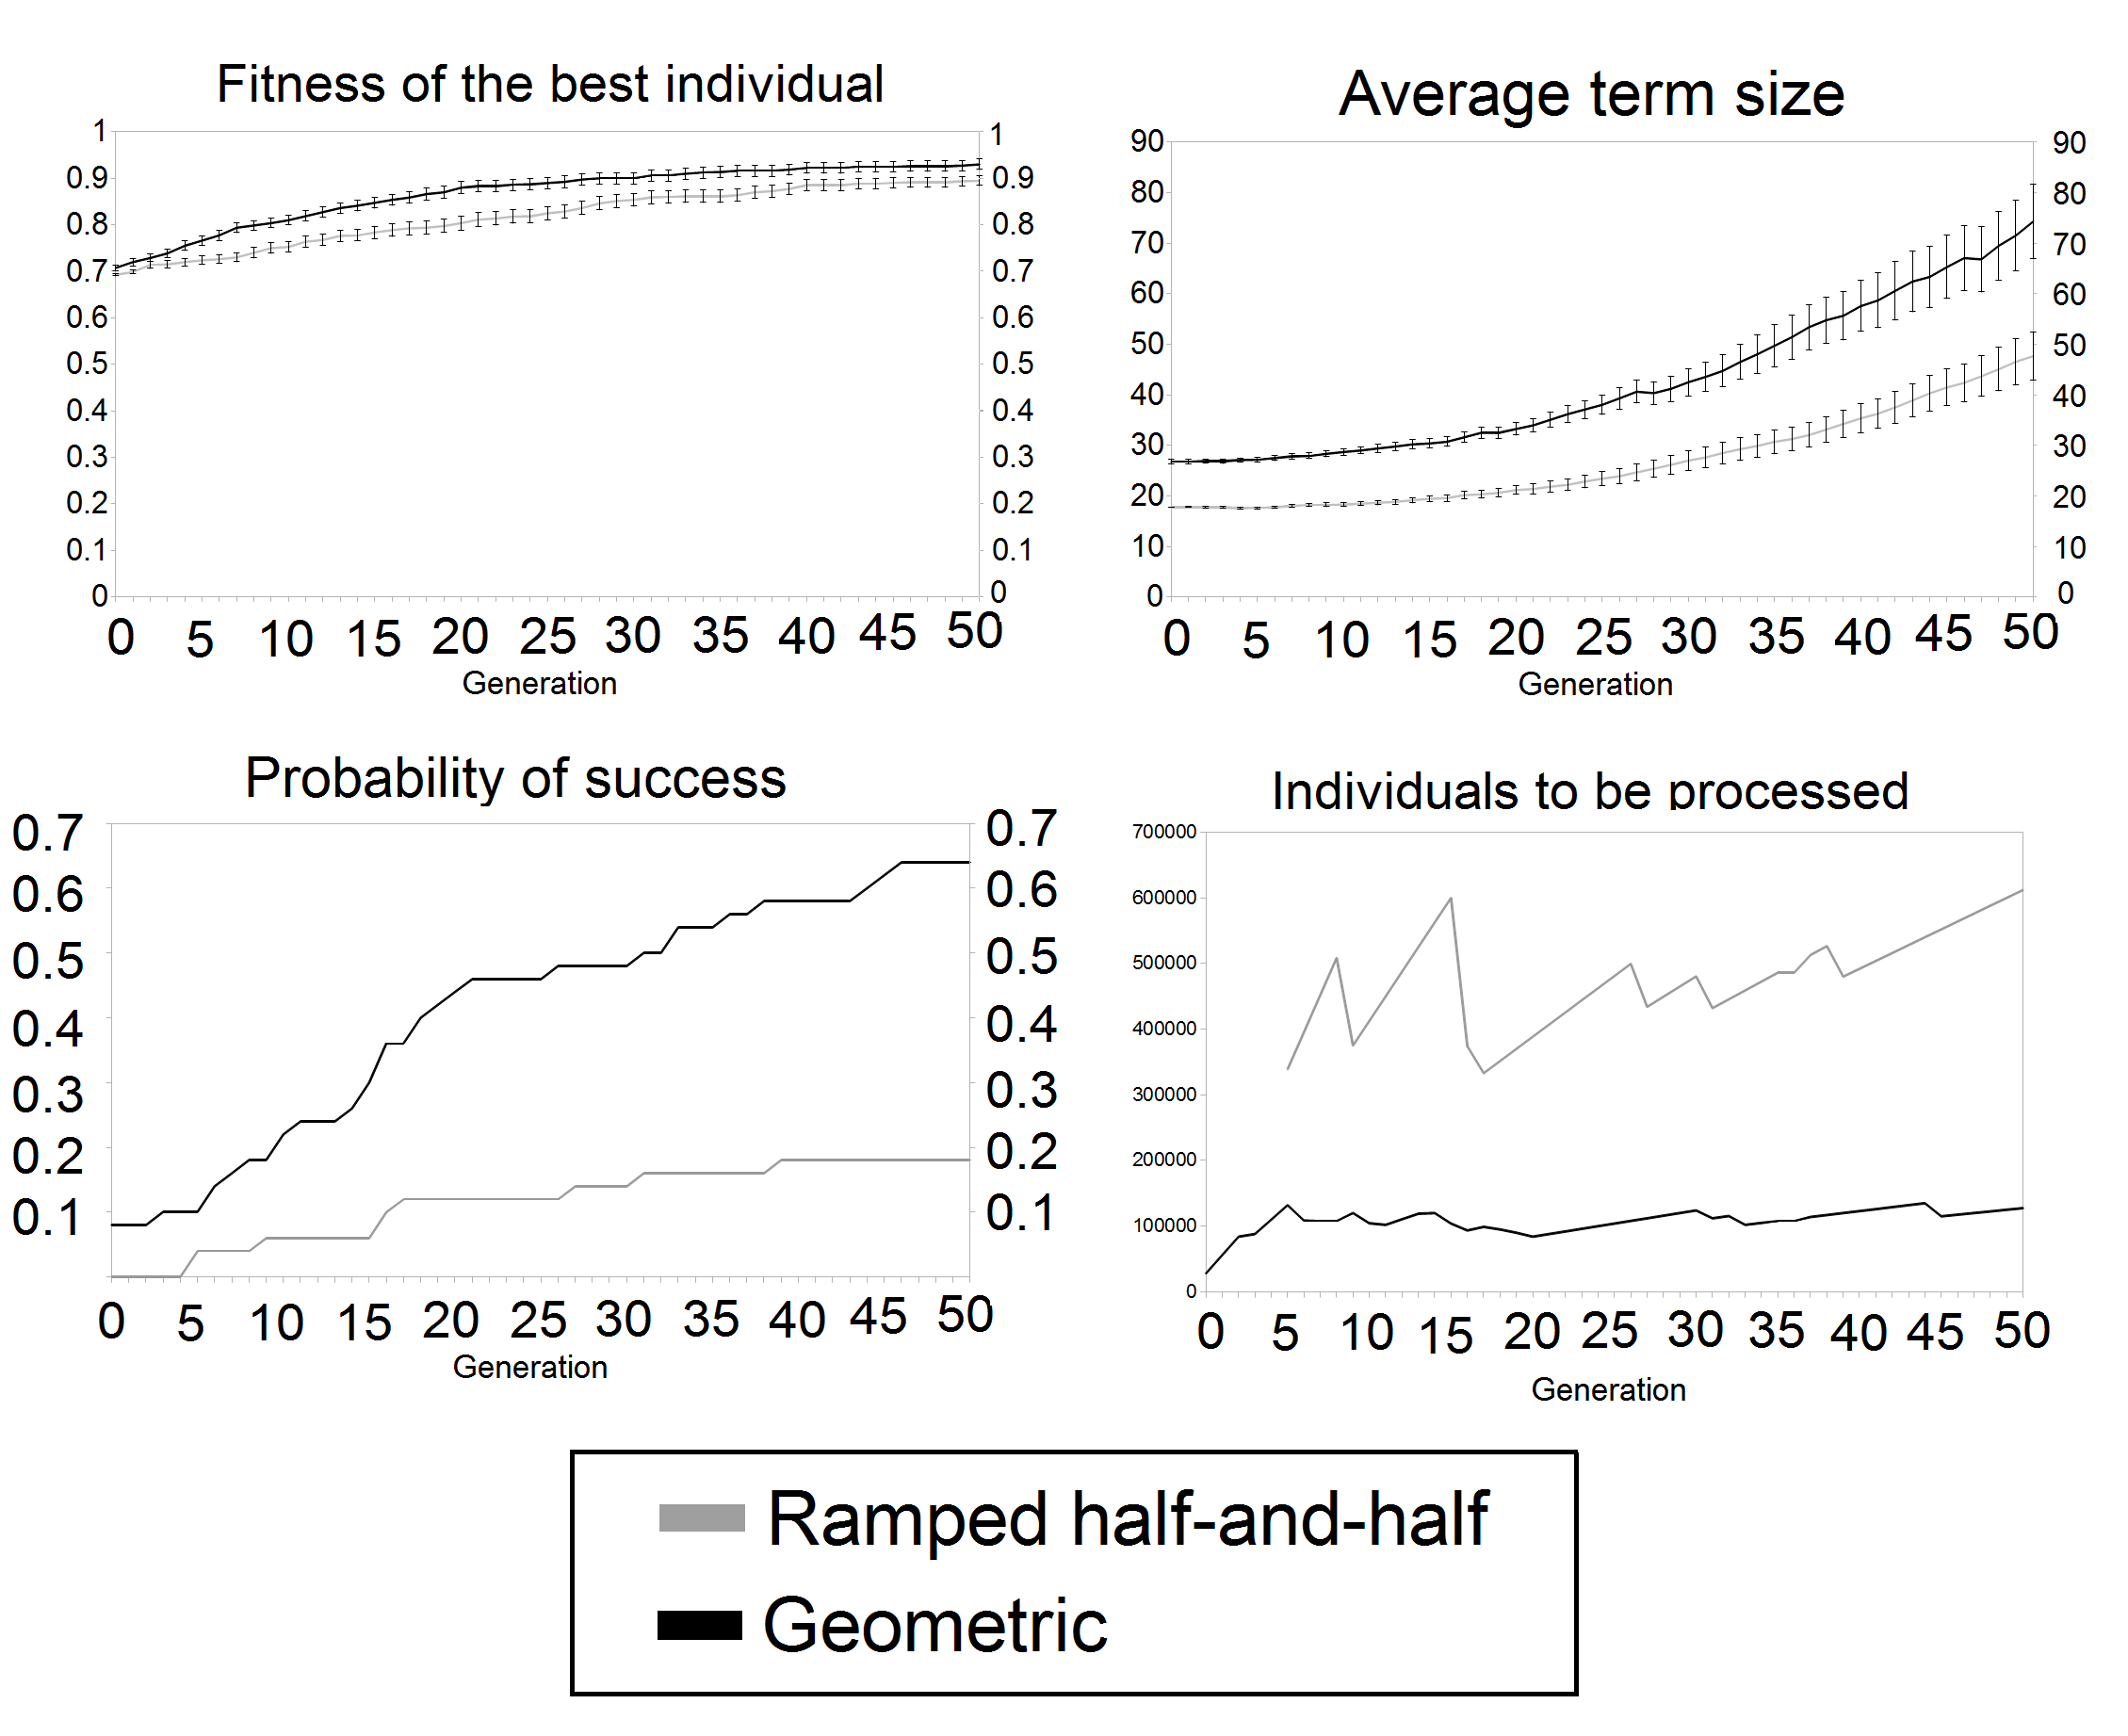
\includegraphics[scale=0.251]{grafy/EP.PNG}
\end{figure}

\begin{table}[t]
\centering
\begin{tabular}{|l|cc|}
\hline
& Unpacking & Hybrid \\
\hline
Mean & 0.935000	& 0.930000 \\
SD	 & 0.066768	& 0.078490 \\
SEM	 & 0.009442	& 0.011100 \\
N	 & 50    & 50    \\
\hline
t-value &  0.3431 & $\alpha = 0.05$\\
p-value &  0.7323 &  \textbf{Not statistically significant}\\
\hline
\end{tabular}
\caption{Statistical analysis.}
\end{table}~\\

Figure~1 shows results of this experiments. 
Table~1 summarizes statistical analysis
of the fitness values of the best individuals of the run 
(\textit{p-value} $ = 0.7323$).  
According to this analysis both crossovers performed about the same;
by conventional criteria, this difference is considered to be not 
statistically significant.

The \textit{unpacking} crossover scored 23/50 (46\%) success rate. 
Minimal $I(M,i,z)$ was in generation 0 with 114,000 individuals to be processed.
The average individual size for generation 50 was 83.1.
The experiment took 388 minutes.

The \textit{hybrid} crossover scored 32/50 (64\%) success rate. 
Minimal $I(M,i,z)$ was in generation 0 with 28,000 individuals to be processed.
The average individual size for generation 50 was 74.3.
The experiment took 33 minutes.

Comparison with other results is summarized in table 2.


\begin{table}[t]
\centering
\begin{tabular}{|l|c|}
\hline
GP approach &  $I(M,i,z)$ \\
\hline
PolyGP                 &  14,000       \\
\textbf{Our approach (hybrid)}&  \textbf{28,000} \\
GP with Combinators	   &  58,616        \\
GP with Iteration      &  60,000       \\
\textbf{Our approach (unpacking)}&  \textbf{114,000} \\
Generic GP	           &  220,000      \\
OOGP	               &  680,000      \\
GP with ADFs           &1,440,000      \\
\hline
\end{tabular}
\caption{Results comparison.}
\end{table}~\\


\section{Conclusions}
\label{conclusions}

We have presented two approaches to crossover for typed GP over lambda terms. The first one (\textit{hybrid}) transforms all generated individuals into combinator terms at the end of generation phase. The second crossover approach (\textit{unpacking}) uses the lambda term representation during the whole run, except for the temporary phases during the crossover. We have compared their relative performance on even parity problem. It shows that the first one is performing the same or better in all observed metrics. This was surprising result for us.

According to comparison of "individuals to be processed" metric our GP approach is performing better than the GP system presented in \cite{kes} and worse than the one presented in \cite{yu01}. By observation of typical solution which is often some modification of \texttt{foldr xor False inputList} one sees that an important task for GP here is to create \texttt{xor} function. This is the advantage for the more specialized term representation used in \cite{yu01}, which 
restricts the use of outer variables. 
It is also fair to say, that this popular metric (in which the comparison data are available) is somehow problematic, since it is prone to have large variation across various instances of the same experiment \cite{luke2002perfect}. As is also visible from our results; both our approaches scored best in generation 0 thus the result depended only on the generation method which those two approaches shared, yet the individuals to be processed estimates are quite different.

In the future work, we would like to accompany our theoretical results concerning relations of generating procedure and reductions described in this paper with experimental results.

In this paper we touched varied aspects of the two lambda calculus concepts -- reductions and abstraction elimination -- in the hope that it will shed some more
light on the promising intersection of lambda calculus and genetic programming.



%\red{
%možná zde zmínit tohle   
%(b) úspornost - abstrakce eliminací produkuje 
%    termy až kvadraticky větší než je původní 
%    term. Dá se očekávat, že i při přímém generování je použití kombinátorů 
%    míň úsporný (proměná se může bez velký námahy objevit v hluboko vnořeném
%    podtermu velmi jednoduše, zatímco pomocí kombinátorů se její hodnota musí        
%    do takto vnořeného podtermu složitě dopravit).
%(c) použití kombů vyžaduje silnější typovej sytém - 
%    kombinátory musej bejt polymorfní a přidáváme je do stavební sady,
%    lambdy v pohodě běžej na simply typed lc. 
%(d) použití proměnných je typické pro lidi, proto by se mohlo sát že
%    i programy generovaný systémem kterej s proměnejma počitá budou o něco 
%    "lidštější" 
%}


%ACKNOWLEDGMENTS are optional
\section{Acknowledgments}

Tomáš Křen has been partially supported by the project GA ČR P202/10/1333 and by the SVV project number 260~104. Roman Neruda has been partially supported by The Ministry of Education of the Czech Republic project COST LD 13002.

%This section is optional; it is a location for you to acknowledge grants, funding, editing assistance and what have you.  In the present case, for example, the authors would like to thank Gerald Murray of ACM for his help in codifying this \textit{Author's Guide} and the \textbf{.cls} and \textbf{.tex} files that it describes.

%\section{Osnova}
%\begin{lizt}
%& Jak reprezentovat stromy programu pro GP?
%  && Reprezentace v klasickym kozovy je S-expression.
%  && Nebo mužem používat kombinátory jako 
%     Briggs a O’Neil (to si myslim je jakoby 
%     hlavní konkurence, vuči který by to chtělo obhájit)
%  && Lambda termy a jejich awesomeness
%& \textbf{Povídaní o redukcích}
%& Povídání o lnf
%  && že lnf je přirozený rozšíření s-exprešnu do lambda 
%     kalkulu vlastnosti termu v lnf 
%     &&& proč je eta redukovat (eta redukcí lnf dostanem 
%         beta-eta-nf a že nemusíme beta redukovat pač se to tim nerozbyje)
%& Generování
%  && Generování gramatikou
%  && Gramatika pro lnf
%  && (?) Inhabitation trees jako intuitivní model takovýhodle lnf generování
%& Problémy s proměnýma a jak je řešit.
%  && Křížit lambda termy i s proměnejma a abstrakcema, 
%     problémy řešit když nastanou (pomluvit a odsoudit)
%  && Zmenšit prostor termu (tim že někerý nejsme schopný 
%     vygenerovat) s kterým operujeme tak aby křížení už 
%     nebyl problém (to dělá Yu - v těle lambda fce dovoluje 
%     jen použití proměnných z její hlavy)
%  && Převod hned po vygenerování
%  && Převod až při křížení
%     &&& eliminace abstrakcí
%     &&& skřížim
%     &&& vložený kombinátory nahradim odpovídajícím termem
%     &&& celý to redukuju
% & Pokusy (?!)
% & Závěr
%\end{lizt}


%
% The following two commands are all you need in the
% initial runs of your .tex file to
% produce the bibliography for the citations in your paper.
\bibliographystyle{abbrv}
\bibliography{evogp}  % sigproc.bib is the name of the Bibliography in this case
% You must have a proper ".bib" file
%  and remember to run:
% latex bibtex latex latex
% to resolve all references
%
% ACM needs 'a single self-contained file'!
%


% That's all folks!
\end{document}
